This chapter describes how the problems described in section~\ref{sec:problem} have been approached and how the concepts presented in section~\ref{chap:tech_background} result in the technical foundations of the system. This concludes in the high-level design and modules of Rymd and Shuttle.

% TODO Robert: Introduction to the overall system design?

%TODO: Motivate choice of AES-CBC-256 (in implementation?)
%Why RSA and not diffie hellman?

\section{Data storage}
\label{sec:datastorage}
Storage of data is crucial for any file sharing system. Since the data store was to be used by several parts of the application the demands for the module's interface had to be as general as possible, adhering to a standard CRUD\footnote{Create–Read–Update–Delete} interface, including methods for creating, fetching, updating and deleting records in the store.

There are essentially four alternatives for persisting data on the client:

\begin{itemize}
\item LocalStorage (Web Storage)
\item IndexedDB
\item WebSQL
\item FileSystem API
\end{itemize}

LocalStorage is included in the HTML5 Web Storage specification \cite{WebStorage:Online} and is a basic key-value store with a simplistic API. It is supported across all major browsers and has a maximum storage limit of 5 megabytes. The latter was a deal-breaker since the product would have to support larger files than could possibly fit into that space. Further, LocalStorage does not support complex structures and indexing, and storing different data types is complicated and needs manual serialization and deserialization. Thus this solution was immediately rejected.

IndexedDB and WebSQL are both client side databases and more sophisticated storage solutions than LocalStorage. WebSQL is supported by Google Chrome, Apple Safari (desktop and iOS), Opera and Android. The specification is no longer maintained by W3C \cite{WebSQL:Online} and will probably be deprecated on all browsers in the future. IndexedDB is supported by all major browsers except for Safari (desktop and iOS) and is a Candidate Recommendation by W3C \cite{IndexedDB:Online}. Arbitrary types of data can be stored in the database, such as strings, numbers, Javascript objects, and raw binary data.

The last alternative, The FileSystem API, is a collection of methods for reading and writing to a sandboxed file system from a browser with client Javascript code. It is a very early standard, being currently only supported by Google Chrome and Opera, and has the status of Working Draft by W3C \cite{FileSystem:Online}. While FileSystem has good performance for larger files and a well-performing asynchronous API, it lacks support for indexing and search. Mozilla seems to have no plans on implementing FileSystem for Firefox \cite{MozillaFileSystem:Online}. In April 2014 it was announced on the Web Applications Working Group mailing list that the specification should be considered dead, since other browser vendors have had no interest in implementing it\cite{FileSystemMailingList:Online}.

All of the mentioned technologies are sandboxed: the data is tied to a single origin (\emph{http://test.domain.com} for instance). All future access to the data must come from that domain (this includes the protocol and port number as well). The browser also limits the maximum allowed storage size – the quota. The quota is different for each storage mechanism, and the browser typically asks the user with a dialog if they want to let the app exceed the quota.

\begin{table}
    \begin{tabular}{|l|l|l|l|l|}
    \hline
                       & IndexedDB & WebSQL & File System & LocalStorage \\ \hline
    Google Chrome 34               & Yes       & Yes    & Yes  & Yes                      \\ \hline
    Mozilla Firefox 29             & Yes       & \cellcolor{red}No  & \cellcolor{red}No   & Yes                        \\ \hline
    Apple Safari 7                & \cellcolor{red}No        & Yes  & \cellcolor{red}No    & Yes                        \\ \hline
    Opera 20                       & Yes       & Yes    & Yes  & Yes                      \\ \hline
    Microsoft Internet Explorer 11 & Yes       & \cellcolor{red}No  & \cellcolor{red}No   & Yes                        \\ \hline
    \end{tabular}
    \caption {Browser support for selected HTML5 APIs at the time of writing}
\end{table}

The conclusion was to use IndexedDB for persisted resource storage. It was chosen because of its support by Google Chrome, Internet Explorer and Firefox, and due to the fact that it is actively maintained (while WebSQL is not). Users of the Safari browser will not be able to utilize the product, but considering the project's overall direction with regards to experimental technologies, this is negligible.

\section{Peer-to-peer communication}

Even though there are two projects which seeks to enable peer-to-peer communication in the browser - WebRTC and CU-RTC-Web - the only viable alternative for the time being is WebRTC. The project is under development by the organizations W3C and IETF and is supported by the current versions of Chrome, Firefox and Opera. CU-RTC-Web on the other hand is not supported by either W3C or IETF and is not implemented in any browsers.

For the project's intent of file sharing, the RTCPeerConnection and RTCDataChannel API were found to be most relevant. By using these APIs in conjuction arbitrary data can be sent peer-to-peer. Relating back to the project goals regarding privacy and security it is also convenient that data transfers are encrypted according to the DTLS protocol.

\section{Peer identity verification}
\label{sec:authorization}
One of the main issues to be resolved in a project of this nature is that of distribution of cryptographic keys. For a truly decentralized system, it is not acceptable to adapt a CA-centered approach, because of the high level of trust that is put in central authorities. While a Web of Trust is interesting, it might be too cumbersome for users. This issue is addressed in "Zooko's Triangle" (See figure~\ref{fig:zooko}), stating that no system assigning names to participants in a network can have the property that names are secure, decentralized and meaningful at the same time\cite{Zooko:2001:Online}. The conjecture has since been proven false by the design of systems such as the blockchain of the cryptocurrency Namecoin, which effectively acts as a cryptographically secured distributed hash table (DHT) with unique keys. Users can reserve a name and assign to it a value of their choice at the cost of a small amount of the Namecoin currency (currently 0.01 NMC \cite{Namecoin:2014:Online}, which is roughly equivalent to 0.03 USD \cite{CryptoCoinCharts:2014:Online}). Ethereum, which was announced just a couple of weeks before the start of this project, extends this by their scripting language which not only allows storage of arbitrary data in the blockchain, but can also be scripted with a Turing complete programming language and can therefore be used to implement arbitrary systems. A system like Ethereum could be very interesting to explore for a project like Rymd, but it is still in such an early stage that it is deemed too unstable to be useful at this point. Namecoin is currently considered a good candidate for key distribution.

Rymd therefore utilizes Namecoin for storage of keys to achieve all of these goals: The distributed nature of cryptocurrencies makes it decentralized; peers can choose their own names (identities), giving meaningful names; the blockchain-based approach makes it secure. Additionally, the small monetary fee required to register a name prevents massive name-squatting. However, there are practical limitations and consequences associated with this approach. The monetary cost associated with the insertion of a new value means that key insertion needs to be handled outside of Rymd. That updates can take a significant amount of time to propagate over the network (up to several hours) is another issue, but since insertion or updates of keys should happen very seldomly, this should be acceptable. Most importantly, since Namecoin (or any other currently existing cryptocurrency for that matter) communicates using their own binary data protocol\cite{BitcoinSource:2014:Online}, web applications can not interact directly with the blockchain to fetch this information before a mutual peer-to-peer authenticated connection is established. As a consequence, a service that acts as a bridge between Rymd and the blockchain is needed.

\begin{figure}[ht]
\centering
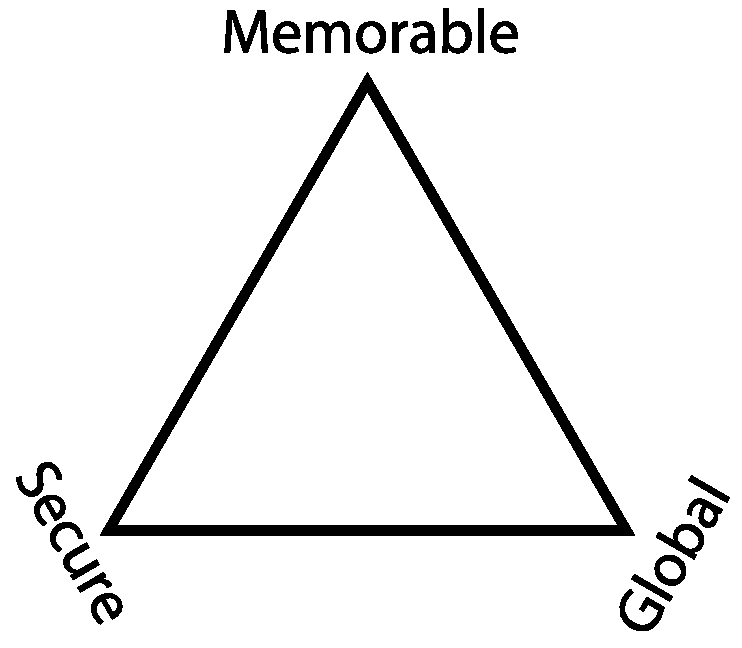
\includegraphics[width=\textwidth,height=0.2\paperheight,keepaspectratio
]{figures/Zooko_s_Triangle}
\caption{Zooko's Triangle, with the edges representing the achievable combinations of features \cite{WikiMedia:2006}}
\label{fig:zooko}
\end{figure}

Once a key distribution scheme has been established, an authentication scheme needs to be determined. There are several schemes for authentication using public-key cryptography. Among these are Otway Rees (not mutual, attacks exist\cite{Wang:2000}), Wide Mouth Frog\cite{Burrows:1990} (depends on timestamps), and Needham-Schroeder\cite{Needham:1978}. Of the ones examined, Needham-Schroeder stood out as simple to implement since it does not utilize symmetric keys or timestamps, while it provides mutual authentication. Consider the scenario where $A$ wants to authenticate to $B$, assuming that they have already exchanged public keys $K_{PA}$ and $K_{PB}$. Then the Needham-Schroeder protocol flows like below:

\begin{description}
  \item[$A \rightarrow B: \{N_A, A\}_{K_{PB}}$] $A$ generates a random nonce $N_A$, encrypts it together with their identity and sends it to $B$.
  \item[$B \rightarrow A: \{N_A, N_B\}_{K_{PA}}$] $B$ responds by generating their own nonce $N_B$, encrypts it together with $N_A$ and sends it back to $A$. By replying with $N_A$, they prove that they possess the private key corresponding to $KP_B$.
  \item[$A \rightarrow B: \{N_B\}_{K_{PB}}$] $A$ replies with $N_B$. The proof works in the same manner as for $B$. $A$ and $B$ are now mutually authenticated.
\end{description}

In 1995, Gavin Lowe described a man-in-the-middle attack on the protocol where an adversary that can initiate a session with one party can then pose as that party when communicating with a third party\cite{Lowe:1995}. Lowe also proposed a fix to this vulnerability and this amended \emph{Needham-Schroeder-Lowe protocol} presented below is what Rymd utilizes for authentication.

\begin{description}
  \item[$A \rightarrow B: \{N_A, A\}_{K_{PB}}$]
  \item[$B \rightarrow A: \{N_A, N_B, B\}_{K_{PA}}$] $B$ also includes their identity to make sure that this message can not be reused by other parties posing as someone else.
  \item[$A \rightarrow B: \{N_B\}_{K_{PB}}$]
\end{description}

\section{Decentralization}
Since the system utilizes the Namecoin blockchain for storage of public keys, there is an issue of how to interface web applications with the blockchain without putting too much trust in the HTTP/cryptocurrency gateway. Users could host their own gateways or retrieve or verify keys manually through their own Namecoin clients. Additionally, as previously stated, the initial insertion of the key requires monetary resources and is something that should be solved outside of Rymd. Users can either provide their existing keys and identity to Rymd or let Rymd generate a new pair of keys and manually insert the public part in the DHT of choice.
While the public key can be stored in a DHT, private keys need to be stored securely on each client, preferably without giving client code any direct access to the raw keys.

\section{Creation and transfers of resources}
\label{sec:creationofresources}
First, we address the question of how to identify resources. That identifiers should be memorable, secure and unique holds not only for users, but also for resources. Since Namecoin is being used for storage of public keys of users, it is therefore natural to consider using a cryptocurrency for resources, too. However, the practical limitations on insertion and updates becomes a much bigger issue here, since resources are created and updated in a much higher frequency than users register or update their public keys. These practical issues would make such a system practically unusable. Therefore, the idea of using any current cryptocurrency blockchain for storing anything resource-related was discarded. File names are not even close to unique and disclose unnecessary information, should an adversary without the corresponding secret key get hold of an encrypted resource. Since resources are communicated peer-to-peer, the issue of malicious resource identifier collision attacks becomes negligible since users would have first-hand contact with peers that they trust and can verifiy the identity of. Therefore, resources are simply identified by a randomly GUID generated at the time of resource creation.

Full access to a resource implies possession of three things: the encrypted resource data, the cryptographic key used to encrypt said data and the metadata describing the resource. The creation of a new resource is done as follows:

\begin{description}
  \item[Generation of metadata] Metadata consists of resource name, author identity, MIME type, a randomly generated GUID, incrementing file version (always $1$ in the case of new resource) and a timestamp.
  \item[Generation of resource-specific symmetric cryptographic key] In the default implementation, a 256 bit AES-CBC key is used.
  \item[Encryption of the resource data using the resource key]
  \item[Calculation of resource hash based on the metadata and encrypted data] The hash is then added to the metadata.
  \item[Combination of metadata and encrypted data into the internal representation of the resource]
  \item[Saving of key to local key store]
\end{description}

To save a resource locally, a user-specific symmetric \emph{master key}, generated at the time of first access, is used to encrypt the metadata before saving it and the encrypted resource data to a local resource store.

The exact flow involved in a transfer depends on the implementing application. Generally (and in Shuttle), the metadata and the encrypted data are transferred separately - maybe even from separate peers. Therefore the hash is important to verify the integrity of the encrypted data. Resource IDs and hashes could also be communicated via trusted channels outside of Rymd, for example on web pages or via e-mail. Once again, verification of integrity and authenticity of resources are achieved by verifying the hash. It is vital that a sufficiently secure hashing algorithm is used; MD5, which used to be the de-facto standard for generating file checksums, has been proven to be weak and contain vulnerabilities to the extent where checksum collisions are too easy to generate \cite{MD5Broken:Online}. SHA-1 has for some time been recommended for verification of data integrity, but due to theoretical collision attacks and advances in computational capabilities, the U.S. government currently recommends against the use of SHA-1 for applications that require collision resistance\cite{NIST:2012}. In the default Rymd implementation, the superceding SHA-256 algorithm is used. This gives a strong protection while avoiding the computational overhead of e.g. SHA-512. Note that hashing provides message integrity, but not authentication (establishment of author). This could be established by letting the author of the resource sign the hash with their private key. Peers on the receiving end could then verify the signature using the author's public key. Establishing resource authentication has not been considered a main goal of Rymd and this functionality is therefore not (yet) implemented.

The metadata and resource data are handled separately in Rymd and the communication flow will differ depending on the implementing application. Generally, the metadata will be shared with trusted peers to allow them to decrypt the resource. The encrypted resource can be shared freely since possession of the key is required to make anything useful from it. In this way untrusted peers could help facilitate transfers of resources in a distributed fashion. In the example implementation Shuttle, file sharing is initiated from the sharing end. Consider the case where Bob wishes to share a resource with Alice (assuming both Alice and Bob are already connected to the network):

\begin{figure}[ht]
\centering
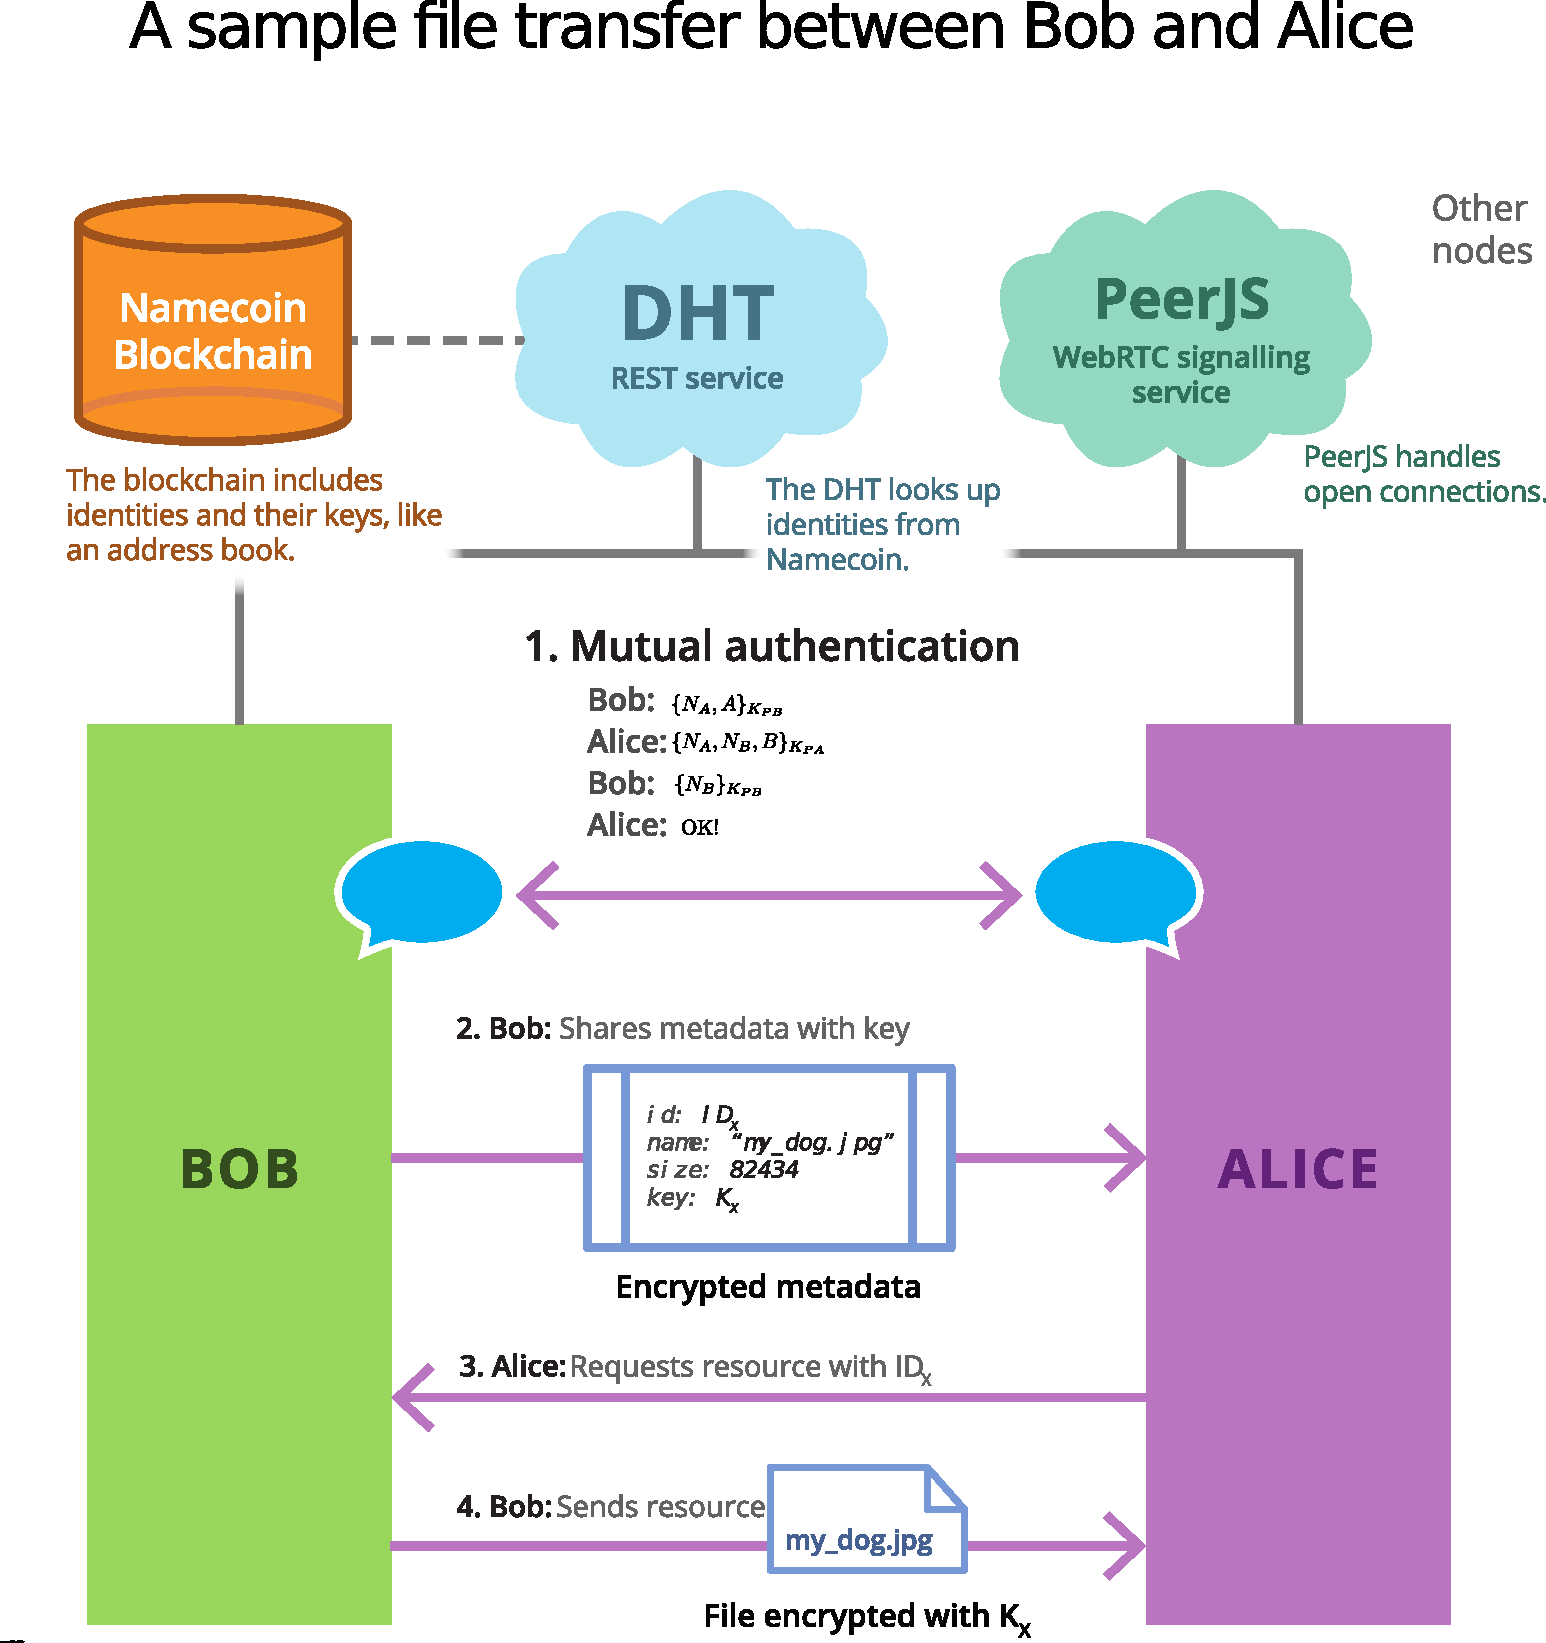
\includegraphics[width=\textwidth,height=0.4\paperheight,keepaspectratio
]{figures/flow}
\caption{The flow involved in Bob sharing a resource with Alice}
\label{fig:flow}
\end{figure}
\begin{enumerate}
  \item Bob requests Alice's public key and endpoint IDs from the DHT.
  \item Bob initiates a connection with Alice and they are mutually authenticated. This process is described in~\ref{sec:authorization}.
  \item Bob sends the metadata and key for the resource to Alice.
  \item Alice creates a new resource as described above, but without the encrypted data, and saves it to her data store.
  \item Alice requests the resource data from Bob.
  \item Bob sends the encrypted resource data to Alice.
  \item Alice adds the encrypted data to the resource and saves it to the data store.
  \item When Alice wants to access the resource, she decrypts it.
\end{enumerate}


\section{Modules in Rymd}

% TODO Robin: Describe our concrete modules better here. This section *has* to describe how
% *we* used modularity in our project.

The core Rymd library contains no implementation meant to deal with a problem area but rather acts as the central hub with workflows that binds all parts together. The library is divided into modules that separates complex areas of the application – areas that are most likely to change independently over time – into well defined and easily exchangeble \emph{modules}. With key features being implemented with technologies from everchanging fields at the web's forefront, this modular design was imperitive in order to make the system maintainable (as explained in section \ref{sec:modularity}). Key functionality were extracted into the following modules along their described responsibilites:

\begin{description}
  \item [Cryptography] Handles encryption, decryption, signing and verification as well as key generation and hashing. 
  \item [Peer-to-peer communication] Responsible for setting up initial contact with another peer and maintaining the connection. It also deals with securing this connection through end-to-end encryption.
  \item [DHT interaction] Used to interface with a Distributed Hash Table in order to retrieve peers' public key and ID.
  \item [Data storage] Deals with persisting file data and metadata (as described in section~\ref{sec:creationofresources}) on disk, and this module also provides means of accessing and manipulating the data.
  \item [Key storage] Solves storing and providing access to cryptographic keys.
\end{description}

Rymd is designed to have the modules supplied dynamically through dependency injection.


%Cryptoback.js
\begin{Code}
\begin{lstlisting}[caption={Included database operations}, label={lst:cryptoback}]
 //dependecies cryptoback.js
  var rsa = require('bignumber-jt'),
      Q = require('q');

 //dependecies crypto.js
  var root = this,
    Q = require('q'),
    cryptojs = require('crypto-js'),
    utils = require("./cryptoback");
\end{lstlisting}
\end{Code}
